\chapter{Typing Rules}
\begin{figure}
%TODO move to appendix
\fbox{$\Gamma_{co} \vdash_{co} \gamma : \psi$}
\begin{mathpar}
\inferrule*[right=TyCoVar]
{
    (c : \psi) \in \Gamma_{co}
}
{
    \Gamma_{co} \vdash c : \psi
}
\quad
\inferrule*[right=TyCoAx]
{
    (g \; (\overline{a : k}) : v_1 \sim v_2) \in \Gamma_{co}
}
{
    \Gamma_{co} \vdash g \; \overline{v} : [\overline{a} \mapsto \overline{v}]v_1
    \sim [\overline{a} \mapsto \overline{v}]v_2
}
\\
%CoRefl
\inferrule*[right=TyCoRefl]
{
    ~
}
{
    \Gamma_{co} \vdash \langle v \rangle : v \sim v
}
\quad
%CoSym
\inferrule*[right=TyCoSym]
{
    \Gamma_{co} \vdash \gamma : v_1 \sim v_2
}
{
    \Gamma_{co} \vdash \text{sym} \; \gamma : v_2 \sim v_1
}
\\
%CoTrans
\inferrule*[right=TyCoTrans]
{
    \Gamma_{co} \vdash \gamma_1 : v_1 \sim v_2
    \\
    \Gamma_{co} \vdash \gamma_2 : v_2 \sim v_3
}
{
    \Gamma_{co} \vdash \gamma_1 \fctrans \gamma_2 : v_1 \sim v_3
}
\\
%CoApp
\inferrule*[right=TyCoApp]
{
    \Gamma_{co} \vdash \gamma_1 : v_1 \sim v_2
    \\
    \Gamma_{co} \vdash \gamma_2 : v_3 \sim v_4
}
{
    \Gamma_{co} \vdash \gamma_1 \; \gamma_2 : v_1 \; v_3 \sim v_2 \; v_4
}
\\
%CoLeft
\inferrule*[right=TyCoLeft]
{
    \Gamma_{co} \vdash \gamma : v_1 \; v_2 \sim v_3 \; v_4
}
{
    \Gamma_{co} \vdash \text{left} \; \gamma : v_1 \sim v_3
}
\quad
%CoRight
\inferrule*[right=TyCoRight]
{
    \Gamma_{co} \vdash \gamma : v_1 \; v_2 \sim v_3 \; v_4
}
{
    \Gamma_{co} \vdash \text{right} \; \gamma : v_2 \sim v_4
}
\\
%CoFam
\inferrule*[right=TyCoFam]
{
    \overline{\Gamma_{co} \vdash \gamma : v_1 \sim v_2}
}
{
    \Gamma_{co} \vdash_{co} F(\overline{\gamma}) : F(\overline{v_1}) \sim
    F(\overline{v_2})
}
\quad
%CoAbs
\inferrule*[right=TyCoAbs]
{
    \Gamma_{co}, a : k \vdash_{co} \gamma : v_1 \sim v_2
}
{
    \Gamma_{co} \vdash_{co} \forall a. \; \gamma : \forall. a \; v_1 \sim \forall. a
    \; v_2
}
\\
%CoInst
\inferrule*[right=TyCoInst]
{
    \Gamma_{co} \vdash \forall a. \; \gamma_1 : \forall. a \; v_1 \sim \forall. a
    \; v_2
    \\
    \Gamma_{co} \vdash \gamma_2 : v_3 \sim v_4
}
{
    \Gamma_{co} \vdash \gamma_1 [\gamma_2] : [a \mapsto v_3]v_1 \sim [a \mapsto
    v_4]v_2
}
\\
%CoQual
\inferrule*[right=TyCoQual]
{
    \Gamma_{co} \vdash \gamma : v_1 \sim v_2
}
{
    \Gamma_{co} \vdash \psi \Rightarrow \gamma : (\psi \Rightarrow v_1) \sim
    (\psi \Rightarrow v_2)
}
\\
%CoQual
\inferrule*[right=TyCoQInst]
{
    \Gamma_{co} \vdash \gamma_1 : (\psi \Rightarrow v_1) \sim
    (\psi \Rightarrow v_2)
}
{
    \Gamma_{co} \vdash \gamma_1 @ \gamma_2 : v_1 \sim v_2
}
\end{mathpar}
\caption{Simplified Coercion Typing}
\label{fig:fc-co-type}
\end{figure}

\chapter{Poster}
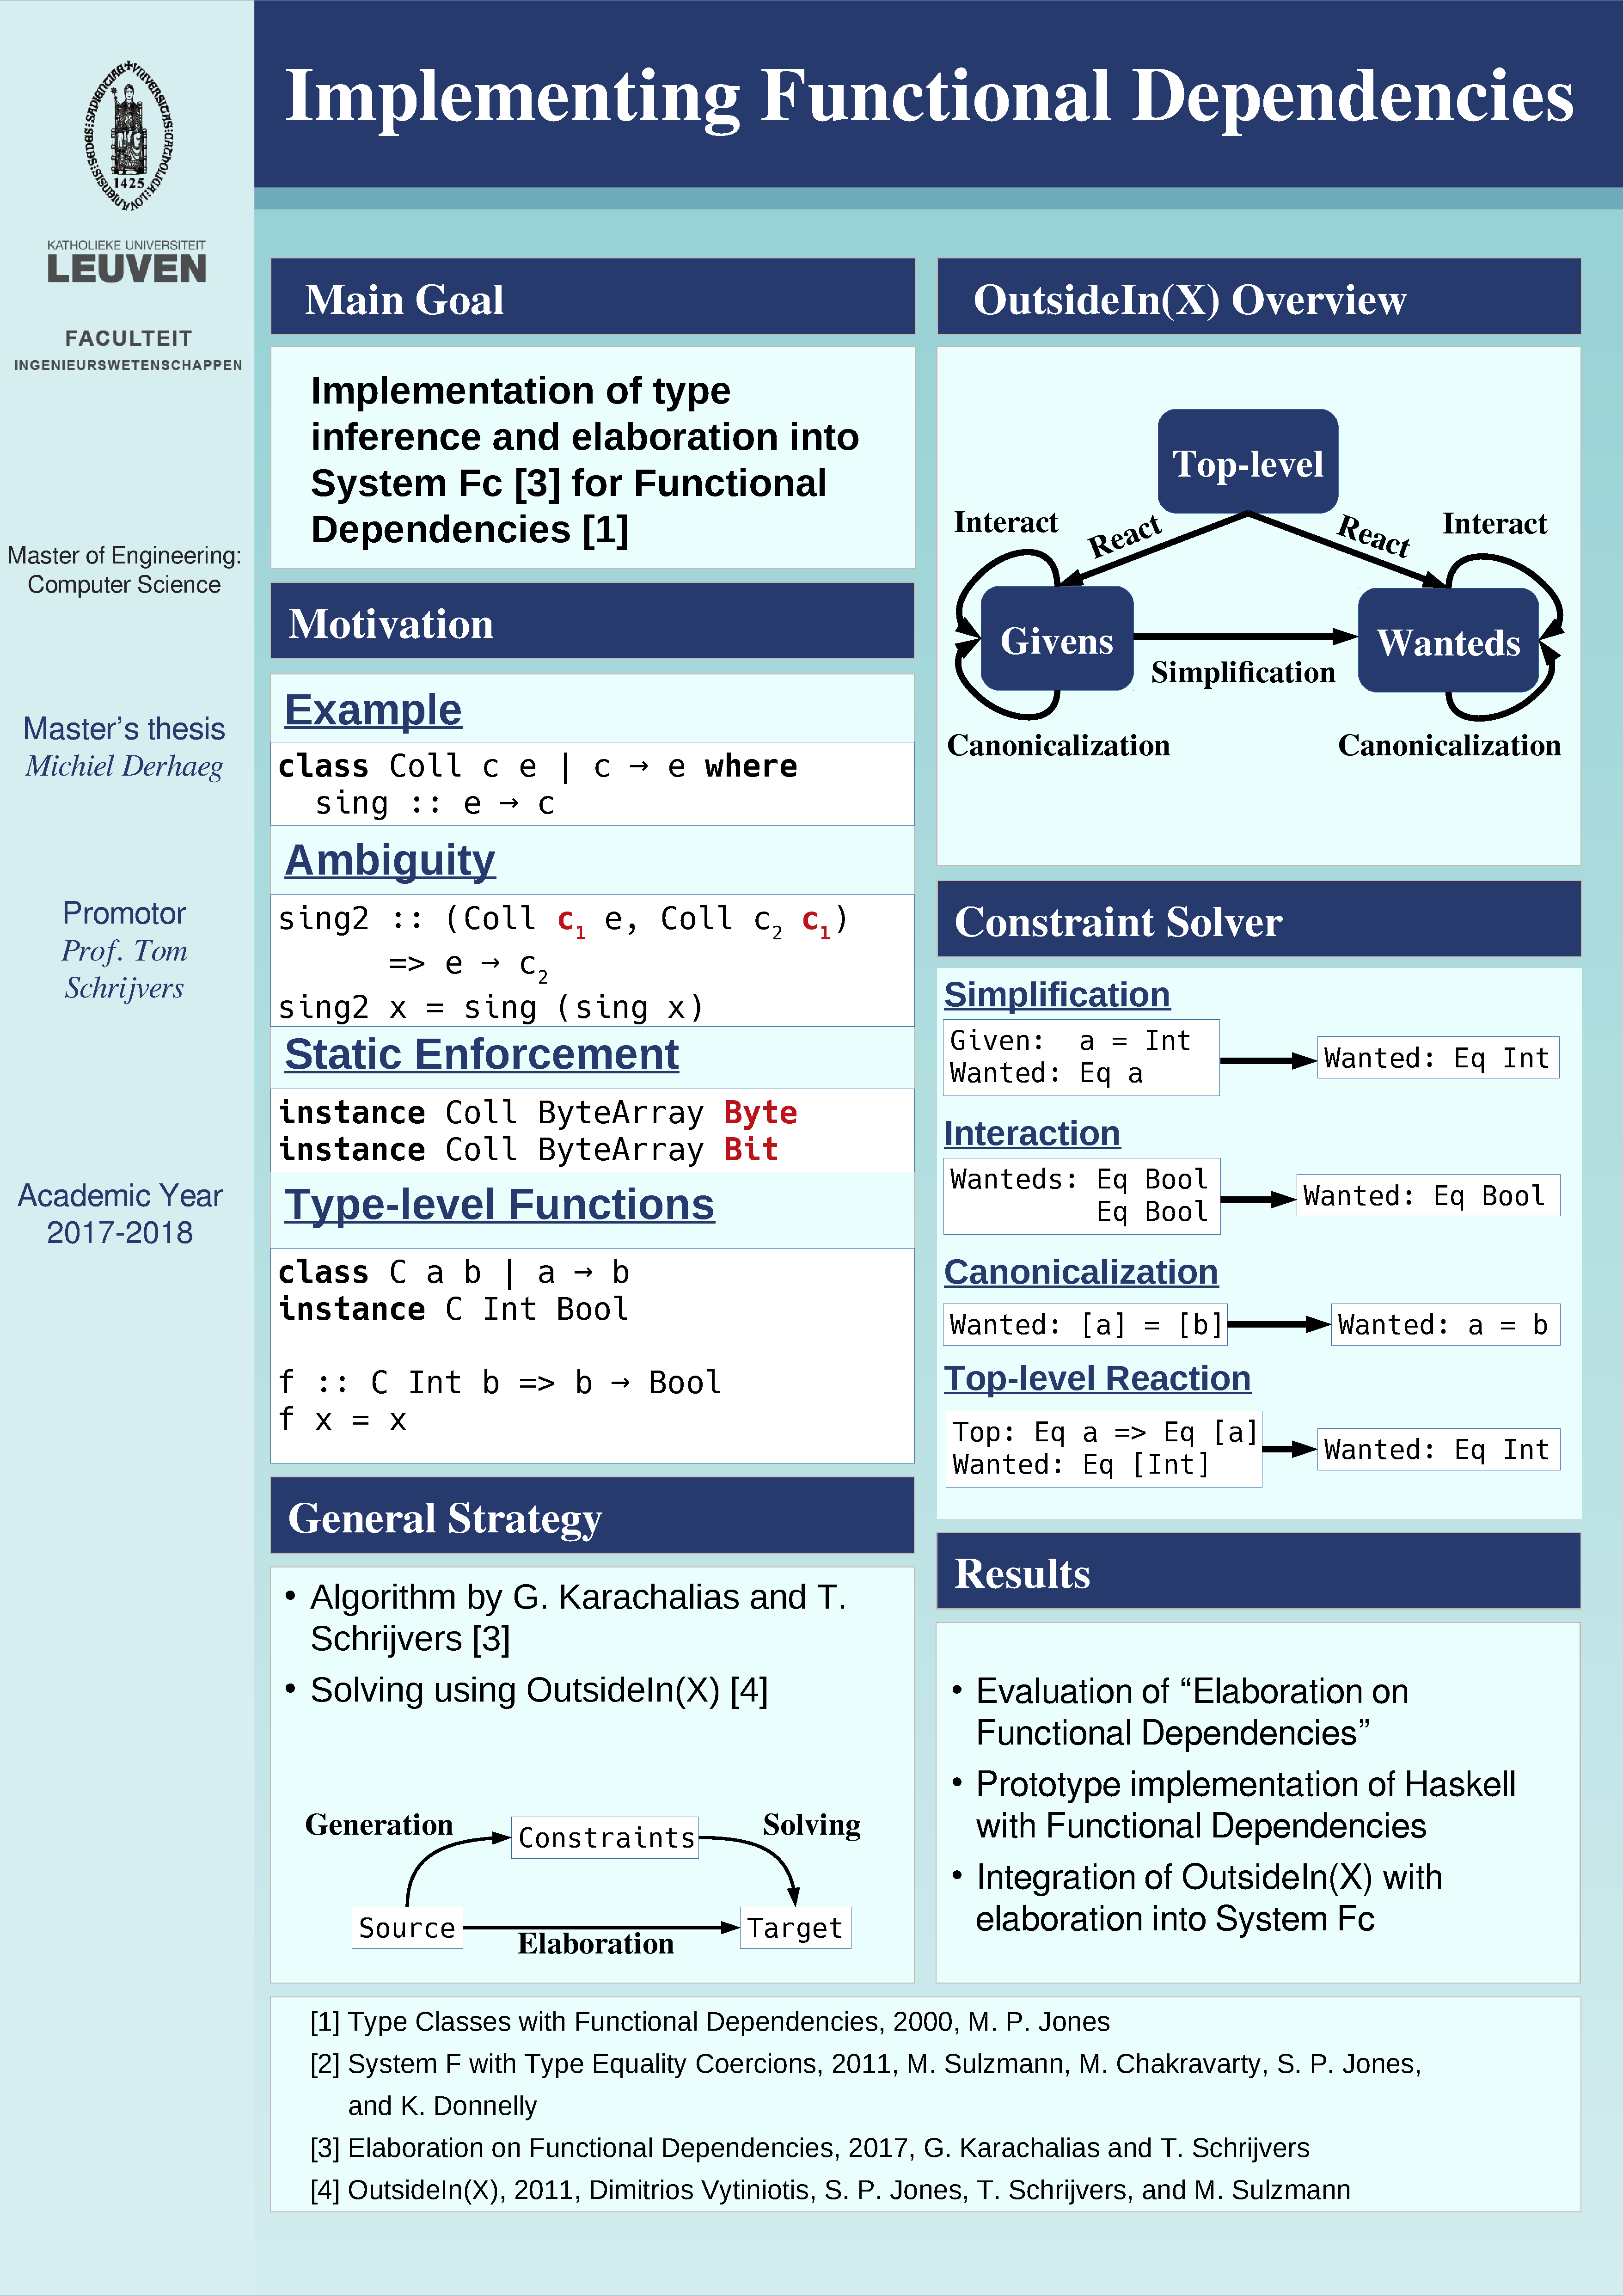
\includepdf[pages=-]{poster.pdf}
